\documentclass[a4paper,12pt]{scrartcl}
\usepackage{graphicx}
\usepackage{luatextra}
%\usepackage{ngerman}
%\usepackage[ngerman]{babel}
%\usepackage{babelbib}
\usepackage{libertine}
\usepackage[EU2]{fontenc}
\usepackage{listings}
\usepackage{color}
\usepackage{url}
\usepackage{bytefield}
%TIKZ--------------------------------------
\usepackage{tikz}
\usetikzlibrary{positioning}
\usetikzlibrary{fit}
\pgfdeclarelayer{background}
\pgfdeclarelayer{belowmain}
\pgfdeclarelayer{foreground}
\pgfsetlayers{background,belowmain,main,foreground}
%------------------------------------------

\newcommand{\haqbus}{ha\textsuperscript{q}\textsubscript{b}us}


\usepackage[pdftex=true,colorlinks=true,linkcolor=black,urlcolor=blue,citecolor=black]{hyperref} 
\title{\haqbus}
\author{C3D2}

\date{}
\makeindex

\definecolor{listinggray}{gray}{0.94}

%anschalten um trennstellen zu sehen:

%\directlua{ show_hyph = function(head) while head do if head.id == 0 or head.id == 1 then show_hyph(head.list) elseif head.id == 7 then local n = node.new("whatsit","pdf_literal") n.mode = 0 n.data = "q 0.3 w 0 2 m 0 7 l S Q" n.next = head.next n.prev = head head.next = n head = n end head = head.next end return true end luatexbase.add_to_callback("post_linebreak_filter",show_hyph,"show_hyph") } 


\begin{document}
\maketitle

\begin{abstract}
This is the first Draft of the haqbus protokoll specification. The haqbus is a field communication system for hackerpsace-automation.
\end{abstract}

\vspace{5cm}
\thispagestyle{empty}
\begin{center}
from Dresden with love by \\
\Large
< < < / > >  \\
\Large
Chaos Computer Club Dresden, c3d2.de 
\end{center}
\biolinumGlyph{Tux} timestamp: \directlua{tex.print(os.time())}  \biolinumGlyph{Tux}
\newpage
\tableofcontents
\newpage
%===============================================================
\section{Introduction}
Standards are cool, everybody should have one!


\section{Usecases and Requirements}

\section{Architectural Overview}
\subsection{Participants in \haqbus}
There are currently 3 roles in which a device could participate in a \haqbus installation:
\begin{enumerate}
\item busmaster
\item passive slave
\item active slave
\end{enumerate}
The busmaster is responsible for doin all the stuff FIXME


\subsection{Layer Specification}
Bus communication is done in 4 different Layers ... or 3 or 5 ?? FIXME
They correspond to the famous ISO/OSI layer model as follows... NOT , so FIXME

%Traditional OSI ISO Stuff:
%Layer 1: physical layer
%Layer 2: data link layer
%Layer 3: network layer
%Layer 4: transport layer
%Layer 5: session layer
%Layer 6: presentation layer
%Layer 7: application layer

\section{Layer one (nameme osi 1)}
TIA/EIA-485 \cite{EIA485}.

Main channel is used with symbolrate of 500000 baud. 



\subsection{Cable Definition}
The used cables are twisted pair cables of 4 pairs plus shielding, that are commonly used for  PentanewsGameshow-buzzers or e.g. in Ethernet cabeling.
The standard suggested is EIA/TIA-568A~\cite{EIA568}.
But rule No. 1 of RFC1925 \cite{RFC1925} applies

\begin{table}
	\centering
	\begin{tabular}{l c l}
		number        & sugested color      & usage \\
		\hline
		1             & white/green stripe  &   FIXME \\
		2             & green solid         &    \\
		3             & white/orange stripe &    \\
		4             & blue solid          &    \\
		5             & white/blue stripe   &    \\
		6             & orange solid        &    \\
		7             & white/brown stripe  &    \\
		8             & brown solid         &    \\
	\end{tabular}
	\caption{%
	Overview of wire asignment  \newline%
	Numbers correspond to pin numbers of an RJ-45 connector as shown in figure~\ref{fig:rj45}.
	}
	\label{tab:wires}
\end{table}

\begin{figure}
	\centering
	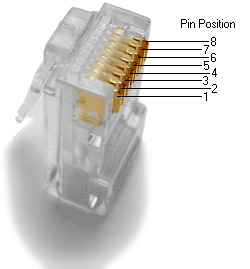
\includegraphics[scale=.7]{png/Rj45plug-8p8c.png}
	\caption{wire numbering on rj45 connector}
	\label{fig:rj45}
\end{figure}

\section{Layer two (nameme osi 2+3)}

\subsection{Bus Checking Phase}
During the bus checking phase the busmaster checks which of all registered devices are still alive. For this the busmaster iterates over its internal table of registered devices and sends a paket of type ASKSTAT~\ref{cp:ASKSTAT} to them.

\subsection{Paket Types}
All Pakets of this layer are at least 4 Bytes long and prefixed with the packet delimiter Byte 0x00. 
Since 0x00 is the paket delimiter any 0 Byte in all other fields of a packet  must be escaped

\subsubsection{ASKSTAT}
Busmaster ask a slave for status
\label{cp:ASKSTAT}
\begin{figure}[h!]
\begin{bytefield}{32}
\bitheader{0,7,8,15,16,23,24,31} \\
\small
\bitbox{8}{Type:ASKSTAT}&\bitbox{8}{check8}&\bitbox{16}{Addr:Reciver}
\end{bytefield}
\end{figure}

\subsubsection{STALIVE}
Normal status answer. Slave sends this, if alive, but nothing to say.
\label{cp:ASKSTAT}
\begin{figure}[h!]
\begin{bytefield}{32}
\bitheader{0,7,8,15,16,23,24,31} \\
\small
\bitbox{8}{Type:STALIVE}&\bitbox{8}{check8}&\bitbox{16}{Addr:Reciver}
\end{bytefield}
\end{figure}


\subsubsection{STALIVPL}
This is similar to STALIVE, but with additional Payload.
\label{cp:ASKSTAT}
\begin{figure}[h!]
\begin{bytefield}{32}
\bitheader{0,7,8,15,16,23,24,31} \\
\small
\bitbox{8}{Type:STALIVPL}&\bitbox{8}{check8}&\bitbox{16}{Addr:Reciver}\\
\wordbox{3}{Payload}\\
\end{bytefield}
%Where the Payload is up to 28 bytes of the form:
%\begin{bytefield}{32}
%\bitbox{8}{len}&\bitbox{24}{data\ldots} \\
 %\bitbox{16 CRC16}\\
%\end{bytefield}
\end{figure}


\subsubsection{ASKSTAT}
\label{cp:ASKSTAT}
\begin{figure}[h!]
\begin{bytefield}{32}
\bitheader{0,7,8,15,16,23,24,31} \\
\small
\bitbox{8}{Type:ASKSTAT}&\bitbox{8}{check8}&\bitbox{16}{Addr:Reciver}
\end{bytefield}
\end{figure}



\section{More Layers}
TODO: specify me!

\newpage
\bibliographystyle{gerplainurl}
%\nocite{LINUX}
\bibliography{spec} 

\end{document}

